% preamble.tex
\documentclass[a4paper,11pt]{book}
\usepackage[english]{babel}
\usepackage{amsmath}
\usepackage{amssymb}
\usepackage{graphicx}
\usepackage{hyperref}
\usepackage{geometry}
\usepackage{booktabs}
\usepackage{amsthm}
\usepackage{enumitem}
\usepackage{caption}
\usepackage{thmtools}
\usepackage[skins]{tcolorbox}
\usepackage{standalone}
\usepackage{tkz-euclide}
\tcbuselibrary{skins, breakable}
\usepackage{parskip}
\usepackage{fancyhdr}
\usepackage{fontawesome5}
\usepackage[x11names,svgnames,table]{xcolor}
\usepackage{setspace}
\usepackage{framed}
\usepackage{tabularx}
\usepackage{fontspec}

\newcommand{\bm}[1]{\symbf{#1}}

\geometry{a4paper, margin=1in}

\fancypagestyle{plain}{
  \fancyhf{}
  \cfoot{\thepage}
  \renewcommand{\headrulewidth}{0pt}
}

\pagestyle{fancy}
\fancyhead{}
\fancyfoot{}
\fancyhead[L]{\nouppercase{\rightmark}}
\fancyhead[R]{\nouppercase{\leftmark}}
\fancyfoot[C]{\thepage}
\renewcommand{\headrulewidth}{0.4pt}
\renewcommand{\footrulewidth}{0pt}

\newtheoremstyle{mythmstyle}%
{}%
{}%
{\itshape}%
{}%
{\bfseries}%
{}%
{ }%
{\thmname{#1}\thmnumber{ #2}%
\thmnote{: #3\addcontentsline{toc}{subsubsection}{{\itshape#1}: #3}}. }

\newcounter{qacount}

% Ambiente Question
\newenvironment{question}{
  \refstepcounter{qacount}
  \vspace{1em} % Spazio sopra la domanda
  \noindent\textbf{Question \theqacount:}\space
}{
  \par % Va a capo alla fine dell'ambiente
}

% Ambiente Answer
\newenvironment{answer}{
  \noindent\textbf{Answer \theqacount:}\space
}{
  \par\vspace{1em}   % Spazio dopo il testo della risposta
  \hrule             % Linea orizzontale di separazione
  \vspace{0.5em}     % Spazio dopo la linea
}

\begin{document}
\chapter*{Basic of EM waves}
\begin{question}
    Describe the Maxwell  equations
\end{question}

\begin{answer}
    % Legge di Faraday
    $\nabla \times \bar{e} = -\frac{\partial \bar{b}}{\partial t}$

    % Legge di Gauss (elettrica)
    $\nabla \cdot \bar{d} = \rho$

    % Legge di Ampère-Maxwell
    $\nabla \times \bar{h} = \bar{j} + \frac{\partial \bar{d}}{\partial t}$

    % Legge di Gauss (magnetica)
    $\nabla \cdot \bar{b} = 0$

    \begin{itemize}
        \item $\bar{e}(\bar{r}, t)$ is ELECTRIC FIELD $[V/m]$
        \item $\bar{d}(\bar{r}, t)$ is the electric flux density $[C/m^2]$
        \item $\bar{h}(\bar{r}, t)$ is MAGNETIC FIELD $[A/m]$
        \item $\bar{b}(\bar{r}, t)$ is MAGNETIC FLUX DENSITY $[T = Wb/m^2]$
        \item $\rho(\bar{r}, t)$ is CHARGE DENSITY $[C/m^3]$
        \item $\bar{J}(\bar{r}, t)$ is ELECTRIC CURRENT DENSITY $[A/m^2]$
        \item $\bar{r} = (x, y, z)$
    \end{itemize}
    Assumptions: $\rho = 0, \vec{J} = 0$
\end{answer}

\begin{question}
    EM fields in harmonic domain
\end{question}

\begin{answer}
    In many cases we can limit the study of EM fields to the harmonic signals. It is convenient to represent fields by their phaser using the following relation:
    \begin{equation}
        \bar{e}(\bar{r}, t) = \text{Re}\left[ \bar{E}(\bar{r}) e^{j\omega t} \right]
    \end{equation}
    In this case we have no electric charges or current. Hence:
    \begin{align*}
        \nabla \times \bar{E} = -j\omega \bar{B} = -j\omega \mu \bar{H}
    \end{align*}
    \begin{align*}
        \nabla \cdot \bar{D} = 0
    \end{align*}
    \begin{align*}
        \nabla \times \bar{H} = j\omega \bar{D} = j\omega \epsilon \bar{E}
    \end{align*}
    \begin{align*}
        \nabla \cdot \bar{B} = 0
    \end{align*}
\end{answer}

\begin{question}
    Describe the constitutive relations
\end{question}

\begin{answer}
    The relation between fields and flux densities depend on the medium where the fields propagate. In general we have:
    \begin{align*}
        \bar{D} = \epsilon \bar{E}
    \end{align*}
    \begin{align*}
        \bar{B} = \mu \bar{H}
    \end{align*}
    where $\epsilon$ is the electric permittivity and $\mu$ is the magnetic permeability of the medium. $[F/m]$ and $[H/m]$ respectively.
\end{answer}

\begin{question}
    Describe Helmholtz equation
\end{question}

\begin{answer}
    The Helmholtz equation is a second-order partial differential equation that describes the propagation of waves in a medium.
    Starting from the Maxwell equations in harmonic domain without charges and currents, we can derive the Helmholtz equation for the electric and magnetic fields.
    \begin{gather*}
        \text{\textbf{Maxwell's Equations (Phasor Form)}} \\
        \begin{aligned}
            \nabla \times \overline{E} & = -j\omega\mu \overline{H}        & \nabla \cdot \overline{E} & = 0 \\
            \nabla \times \overline{H} & = j\omega\varepsilon \overline{E} & \nabla \cdot \overline{H} & = 0
        \end{aligned}
    \end{gather*}

    \begin{gather*}
        \text{\textbf{Derivation of the Helmholtz Equation}} \\
        \text{1) Apply the curl to Faraday's Law:} \\
        \nabla \times (\nabla \times \overline{E}) = \nabla \times (-j\omega\mu \overline{H}) \\
        \\
        \text{2) Due to the linearity of the operator, move the constants outside:} \\
        \nabla \times (\nabla \times \overline{E}) = -j\omega\mu (\nabla \times \overline{H}) \\
        \\
        \text{3) Substitute the curl of } \overline{H} \text{ using the Ampère-Maxwell Law:} \\
        \nabla \times (\nabla \times \overline{E}) = -j\omega\mu (j\omega\varepsilon \overline{E}) \\
        \\
        \text{4) Simplify the constant terms (given that } j^2 = -1\text{):} \\
        \nabla \times (\nabla \times \overline{E}) = \omega^2\mu\varepsilon \overline{E} \\
        \\
        \text{5) Use the vector identity } \nabla \times \nabla \times \overline{A} = \nabla(\nabla \cdot \overline{A}) - \nabla^2\overline{A} \text{:} \\
        \nabla(\nabla \cdot \overline{E}) - \nabla^2\overline{E} = \omega^2\mu\varepsilon \overline{E} \\
        \\
        \text{Since } \nabla \cdot \overline{E} = 0 \text{ in a source-free medium, the gradient term vanishes:} \\
        -\nabla^2\overline{E} = \omega^2\mu\varepsilon \overline{E} \\
        \\
        \text{6) Rearrange the terms to obtain the Helmholtz Equation:} \\
        \nabla^2\overline{E} + \omega^2\mu\varepsilon \overline{E} = 0
    \end{gather*}

    For magnetic field the steps are the same.

\end{answer}

\begin{question}
    What is the advantage of using piecewise homogeneous media?
\end{question}

\begin{answer}
    Piecewise homogeneous is a semplification that allows us to consider $\epsilon$ and $\mu$ as constants in a given region.
    But normally $\epsilon$ and $\mu$ are not constant, so we solve this problem by using boundary conditions.
\end{answer}

\begin{question}
    What are the boundary conditions?
\end{question}

\begin{answer}
    We consider the thin surface between 2 different materials. We define the normal versor $\hat{n}$ .
    \subsection*{For flux densities}
    \begin{itemize}
        \item \textbf{Density of magnetic flux}: normal component is always continuous
              \begin{equation}
                  \hat{n} \cdot (\bar{B}_2 - \bar{B}_1) = 0
              \end{equation}
        \item \textbf{Density of electric flux}: normal component is discontinuous
              \begin{equation}
                  \hat{n} \cdot (\bar{D}_2 - \bar{D}_1) = \rho_s
              \end{equation}
    \end{itemize}
    \subsection*{For fields}
    \begin{itemize}
        \item \textbf{Electric field}: tangential component is always continuous
              \begin{equation}
                  \hat{n} \times (\bar{E}_2 - \bar{E}_1) = 0
              \end{equation}
        \item \textbf{Magnetic field}: tangential component is discontinuous
              \begin{equation}
                  \hat{n} \times (\bar{H}_2 - \bar{H}_1) = \bar{J}_s
              \end{equation}
    \end{itemize}

    For our assumptions, $\rho_s = 0$ and $\bar{J}_s = 0$.
\end{answer}

\begin{question}
    Describe the Poynting vector
\end{question}

\begin{answer}
    In the time domain the Poynting vector is defined as:
    \begin{equation}
        \bar{P}(\bar{r}, t) = \bar{E}(\bar{r}, t) \times \bar{H}(\bar{r}, t)
    \end{equation}
    where $\bar{E}$ is the electric field and $\bar{H}$ is the magnetic field.\\
    While in the harmonic domain we have:
    \begin{equation}
        \bar{P}(\bar{r}) = \frac{1}{2} \bar{E}(\bar{r}) \times \bar{H}^*(\bar{r})
    \end{equation}
    where $\bar{H}^*$ is the complex conjugate of $\bar{H}$.\\
    In other words, it represents the power flow per unit area.

\end{answer}

\begin{question}
    Describe the polarization of EM waves and the polarization plane
\end{question}

\begin{answer}
    A generic sinusoidal EM field can be written as:
    \begin{equation}
        \overline{e}(\overline{r}, t) = \sum_{n=1}^{3 \, \text{dim}} C_n(\overline{r}) \cos(\omega t + \phi_n(\overline{r})) \hat{x}_n = \underbrace{c'(\overline{r}, t)}_{\overline{E}_{\text{Re}}} \cos(\omega t) - \underbrace{c''(\overline{r})}_{\overline{E}_{\text{Im}}} \sin(\omega t)
    \end{equation}
    which clearly shows that the electric vector of a generic sinusoidal field lays at any time on a plane defined by the vectors $\overline{E}_{\text{Re}}$ and $\overline{E}_{\text{Im}}$.

    This is known as polarization plane: constant in time, vary in space.
    The sinusoidal field is periodic, so the curve it describes must be closed. Generally, it is an ellipse.

    This ellipse is described by two components:
    \begin{align}
        \bar{e}'(t) =
        \begin{bmatrix} a \cos(\omega t + \phi) \\ b \sin(\omega t + \phi)
        \end{bmatrix}
    \end{align}

    We that the polarization is:
    \begin{itemize}
        \item Right handed: when the field rotates counterclockwise
        \item Left handed: when the field rotates clockwise
    \end{itemize}
    Two notable cases are:
    \begin{itemize}
        \item Linear polarization: when the ellipse degenerates into a line
        \item Circular polarization: when the ellipse degenerates into a circle ($a=\pm b$)
    \end{itemize}
\end{answer}

\begin{question}
    Describe Jones vector and their utility
\end{question}

\begin{answer}
    It's a bidimensional complex vector which describes a generic sinusoidal EF when represented with respect to its polarization plane.
    The Jones vector reads:
    \begin{equation}
        \bar{J} =
        \begin{bmatrix} a\cos(\delta) + j b \sin(\delta) \\ a\sin(\delta) - j b \cos(\delta)
        \end{bmatrix}
    \end{equation}

    \begin{itemize}
        \item $\Phi$ does not influence the polarization, but it's useful to describe field propagation;
        \item Two polarizations are orthogonal if the corresponding Jones vectors are orthogonal. ($\bar{E}_1 \cdot \bar{E}_2 = 0$)
    \end{itemize}
\end{answer}

\begin{question}
    Describe Stokes vector
\end{question}

\begin{answer}
    Stokes vectors are real vectors which describes a more intuitive geometrical representation of light polarization.
    The Stokes vector reads:
    \begin{equation}
        \vec{S} =
        \begin{bmatrix} S_0 \\ S_1 \\ S_2 \\ S_3
        \end{bmatrix} =
        \begin{bmatrix}
            |E_1|^2 + |E_2|^2       \\
            |E_1|^2 - |E_2|^2       \\
            2 \text{Re} [E_1 E_2^*] \\
            2 \text{Im} [E_1 E_2^*]
        \end{bmatrix} =
        \begin{bmatrix}
            a^2 + b^2                \\
            (a^2 - b^2) \cos 2\delta \\
            (a^2 - b^2) \sin 2\delta \\
            2ab
        \end{bmatrix}
    \end{equation}

    \begin{itemize}
        \item $S_0$ total intensity;
        \item $S_1$ difference in intensities between horizontal and vertical linearly polarized components;
        \item $S_2$ difference in intensities between linearly polarized components oriented at +45° and -45°;
        \item $S_3$ difference in intensities between right and left circularly polarized components
    \end{itemize}
    It does not depend on phase.
    \begin{align}
        S_0 = \sqrt{S_1^2 + S_2^2 + S_3^2}
    \end{align}
    Monochromatic case: $\omega$ is constant.\\
    Also, knowing the redundancy of $S_0$, we can define the unit Stokes vector:
    \begin{align}
        \hat{S} = \begin{bmatrix} S_1 \\ S_2 \\ S_3 \end{bmatrix} =
        \frac{1}{S_0} \begin{bmatrix} S_1 \\ S_2 \\ S_3 \end{bmatrix} =
        \frac{1}{a^2 + b^2} \begin{bmatrix}
                                (a^2 - b^2) \cos 2\delta \\
                                (a^2 - b^2) \sin 2\delta \\
                                2ab
                            \end{bmatrix}
    \end{align}

    which can be further simplified with ellipticity: $\epsilon = \tan^{-1}(b/a)$


    \begin{align}
        % Definizione del parametro di ellitticità
        \tan \epsilon  & = \frac{b}{a}                                                                                                     \\
        % Identità trigonometriche per l'angolo doppio
        \cos 2\epsilon & = \frac{1 - \tan^2 \epsilon}{1 + \tan^2 \epsilon} = \frac{1 - (b/a)^2}{1 + (b/a)^2} = \frac{a^2 - b^2}{a^2 + b^2} \\
        \sin 2\epsilon & = \frac{2 \tan \epsilon}{1 + \tan^2 \epsilon} = \frac{2(b/a)}{1 + (b/a)^2} = \frac{2ab}{a^2 + b^2}                \\
        % Sostituzione nel vettore unitario s_hat
        \hat{s}        & = \frac{1}{a^2 + b^2} \begin{bmatrix} (a^2 - b^2) \cos 2\delta \\ (a^2 - b^2) \sin 2\delta \\ 2ab \end{bmatrix}   \\
        % Risultato finale in coordinate angolari (Sfera di Poincaré)
        \hat{s}        & = \begin{bmatrix} \cos 2\epsilon \cos 2\delta \\ \cos 2\epsilon \sin 2\delta \\ \sin 2\epsilon \end{bmatrix}
    \end{align}
\end{answer}

\begin{question}
    Describe the Poincaré sphere
\end{question}

\begin{answer}
    The unit stokes vector can be geometrically visualized as lying on the surface of a sphere of unit radius. Each point on the sphere represents a different polarization state.

    \begin{align}
        \hat{S} = \begin{bmatrix} \cos 2\epsilon \cos 2\delta \\ \cos 2\epsilon \sin 2\delta \\ \sin 2\epsilon \end{bmatrix}
    \end{align}

    the various polarizations are:
    \begin{itemize}
        \item Equator: linear polarization
        \item North pole: circular polarization right handed
        \item South pole: circular polarization left handed
        \item North hemisphere: elliptical polarization right handed
        \item South hemisphere: elliptical polarization left handed
    \end{itemize}

    \begin{figure}[h]
        \centering
        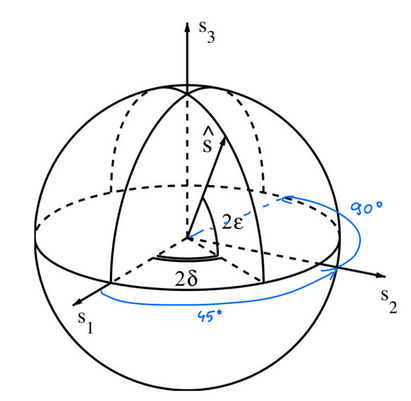
\includegraphics[width=0.5\textwidth]{Pictures/Poincarè-sphere.png}
        \caption{Poincaré sphere}
        \label{fig:poincare_sphere}
    \end{figure}

\end{answer}

\chapter*{Modal theory}
\begin{question}
    What is Total Internal Reflection?
\end{question}

\begin{answer}
    Consider a fiber. We have the core and the cladding. We have to respect two conditions:
    \begin{itemize}
        \item The refractive index of the incidence medium must be greater than the refractive index of the transmission medium ($n_1 > n_2$);
        \item The angle of incidence $\theta_i$ must be greater than the critical angle $\theta_c = \sin^{-1}(n_2/n_1)$.
    \end{itemize}

    When $\theta_i < \theta_c$ we have \textit{uniform trasmitted waves} and $n_1 \sin(\theta_i) = n_2 \sin(\theta_t)$.

\end{answer}


\begin{question}
    Considered a step-index fiber; let us determine the maximum input angle that a ray
    may have so that the ray refracted in the fiber core is guided by TIR.
\end{question}

\begin{answer}
    \begin{itemize}
        \item \textbf{Snell's Law at the input interface (Air to Core):}
              \begin{equation}
                  n_0 \sin \beta_M = n_1 \sin \beta_l \implies \sin \beta_M = n_1 \sqrt{1 - \cos^2 \beta_l} \quad (\text{assuming } n_0 \approx 1)
              \end{equation}

        \item \textbf{Total Internal Reflection (TIR) condition at Core-Cladding interface:}
              The ray is guided if the incidence angle is greater than or equal to the critical angle $\theta_c$:
              \begin{equation}
                  \frac{\pi}{2} - \beta_l \ge \theta_c \implies \cos \beta_l \ge \sin \theta_c
              \end{equation}

        \item \textbf{Critical Angle definition:}
              \begin{equation}
                  \sin \theta_c = \frac{n_2}{n_1}
              \end{equation}

        \item \textbf{Substitution for Maximum Angle ($\beta_M$):}
              Substituting the limiting case $\cos \beta_l = \frac{n_2}{n_1}$ into the first equation:
              \begin{equation}
                  \sin \beta_M = n_1 \sqrt{1 - \left( \frac{n_2}{n_1} \right)^2} = \sqrt{n_1^2 - n_2^2}
              \end{equation}

        \item \textbf{Final Result (Numerical Aperture):}
              \begin{equation}
                  NA = \sin \beta_M = \sqrt{n_1^2 - n_2^2}
              \end{equation}
    \end{itemize}

    Large NA $\implies$ easier to couple light into the fiber, but can cause ISI (modal dispersion).

\end{answer}

\begin{question}
    From S
\end{question}

\begin{answer}

\end{answer}

\end{document}